\documentclass[dvipdfmx,uplatex]{jsarticle}
\title{知識と情報科学第4,5,6回}
\author{
    名前: 長田悠生\\
    学籍番号: 202310330\\
}
\date{2023/7/5}

\usepackage{url}
\usepackage[dvipdfmx]{graphicx}
\usepackage{listings,jvlisting}
\lstset{
  basicstyle={\ttfamily},
  identifierstyle={\small},
  commentstyle={\smallitshape},
  keywordstyle={\small\bfseries},
  ndkeywordstyle={\small},
  stringstyle={\small\ttfamily},
  frame={tb},
  breaklines=true,
  columns=[l]{fullflexible},
  numbers=left,
  xrightmargin=0zw,
  xleftmargin=3zw,
  numberstyle={\scriptsize},
  stepnumber=1,
  numbersep=1zw,
  lineskip=-0.5ex
}

\begin{document}
  \begin{titlepage}
    \maketitle
    \begin{center}
      \textmc{\HUGE \LaTeX}
    \end{center}
    \thispagestyle{empty}
  \end{titlepage}

  \textmc{\LARGE 第4回の要約\\}
  \textmc{
    この講義の内容は、音声・音響処理についてだった。この講義は、人が音声を発する際の仕組み・音声を認識する仕組みについての説明から始まる。
    人の音声器官は、大きく二つに分けられる。発声と調音である。発声は、呼気流から音源を作ることである。調音は、言語としての音響特性を付けることである。
    音源は、三種類に分けられる。声帯の振動音から発せられる音声は、有声音源・口の中の強い狭めによる乱流音は、摩擦性音源・口の中の閉鎖と解放による破裂音は、破裂性音源とされている。
    音響特性は、主に声道の形状によって決まる。声道の形状によって、音の共鳴・反共鳴が発生し、特定の周波数の音が協調・減衰される。
    人はこのようなメカニズムで音声を発し、聞いているという説明をされていた。
    講義の内容は、言語特性(母音と子音)についての話に移る。
    まず、母音についての説明である。母音は、/a/,/i/,/u/,/e/,/o/の音素から構成される音声である。母音の特徴として、口の中に強い狭めを作らないで、声帯振動を伴う。
    また、母音は調音位置(母音の場合は、舌の位置)とあごの開きの二つの変数で音声が決まる。
    次に、子音についての説明である。子音は、/k/,/s/,/t/...などの音素から構成される音声である。子音の特徴として、口の中に強い狭めを作らないで、声帯振動か鼻腔からの空気の流れを伴う。
    また、子音は調音位置(子音の場合は、各音声器官の狭めの位置)と声帯振動の有無と調音様式の三つの変数で音声が決まる。
    講義の内容は、人の聴覚器官についての説明に移る。
    人の聴覚器官で特に重要な役割を果たしている蝸牛についての説明である。蝸牛は、リンパ液で満たされた管の中に基底膜という非常に薄い膜を有している器官である。
    リンパ液の流れが基底膜の振動となって、周波数を感知する仕組みになっている。蝸牛は、低い周波数の分解能が高い周波数の分解能より高いと考えられている。
    人間の音声器官・聴覚器官についての理解を深めることで、より精度の良い音声認識の仕組みの作成につながる。
    講義の内容は、音声認識に移る。
    音声認識は、空気振動を電気振動として受け取り、AD変換の後、特徴量抽出とパターン認識を行うという仕組みで動いている。
    講義では、特に特徴量認識とパターン認識について、より詳しい説明をしていた。
    まず、特徴量抽出の説明をする。
    AD変換によって取得したディジタル信号を各フレームごとにフーリエ変換し、フォルマントの部分を特徴量として取得し、
    各フレームの特徴量の集まりで表現することである。
    次に、パターン認識の説明である。
    パターン認識の手法の主流として、統計的音声認識がある。統計的音声認識は、単語辞書と音響モデルを用いたベイズ推定で確率的に音声認識を
    行うというものである。
    音声認識は、このような仕組みで動いている。
  \\}
  \textmc{\large \\}
  \textmc{\LARGE 第5回の要約\\}
  \textmc{
    この講義は、実現したい問題が解きやすい問題に帰着できない場合の最適化についての説明だった。
    この講義は、数理最適化問題の説明から始まる。
    数理最適化問題とは、問題から目的関数と制約条件を作成することができ、その解を数理最適化アルゴリズムで出力できる問題である。
    しかし、現実に存在する問題のすべてが数理最適化アルゴリズムで出力できる問題であるとは限らない。
    ブラックボックス最適化とは、入力と目的関数による計算結果しかわからない状態の問題について、解を割り出そうとするものである。
    ブラックボックス最適化の具体的な方法として、近似解法やヒューリスティックがある。
    近似解法の手段の一つとして、生物の進化を模倣した進化計算がある。
    進化計算は、評価関数評価による自然淘汰、解集団の交叉と突然変異、世代交代のサイクルによって近似的に解を求めようとするものである。
    現実的に、正確な値を求められなくても近似的な値を求められることは非常に有益なことなのである。
    そのため、ブラックボックス最適化は、現実に存在する様々な数理最適化問題にできない問題に対して、強力に作用する場合があるのだ。
    \\}
  \newpage
  \textmc{\LARGE 第6回の要約\\}
  \textmc{
    この講義は、自動運転に注目した認知工学についての説明だった。
    この講義は、認知工学についての説明から始まる。
    認知工学とは、人間の仕組みを理解し、それを踏まえて人の行動を支援するシステムを設計・構築することを考える学問である。
    次に、自動車事故が起きてしまう理由についての説明を認知工学の観点から行っていた。
    人間の絶対の原理として、人がどんなに頑張ろうとエラーを完全に防げないというものがある。
    この人によるエラーを軽減するためには、人がエラーを起こす仕組みについて理解する必要がある。
    人間の情報処理は、「情報獲得→解析→意思決定→行動」の流れで行われている。
    そして、人間はそれらの情報処理それぞれに注意を払っている。
    しかし、それそれに向けられる注意には限界があることが知られている。
    自動車事故で大きな割合を占めている原因であるドライバーディストラクション(運転に対する注意不足)は、注意の容量の限界を超えた、又は、注意の資源配分をうまくできていないことで発生してしまう。
    運転支援技術は、この問題を解決するために今日まで開発が行われてきた。
    この講義は、ここから運転支援技術についての説明に移る。
    自動車の運転に必要な情報は、大きく三つのレベルに分けられる。それは、戦略的レベル(どういうルートで目的地に行くか)・戦術的レベル(どの車線で行くか)・操作的レベル(周囲とどう安全を確保するか)である。
    戦略的レベルは、カーナビですでに実現されている。戦術的レベルは、コンピュータが行うのは難しい。そのため、現在の運転支援技術は、操作的レベルに対しての技術となっている。
    この講義では、運転支援技術の具体例についていくつか紹介されていた。
    車線をモノクロのピクセルの輝度の変化で割り出し、左右の車線の傾きで、自車の位置を割り出して修正する車線維持機能・電波の反射時間で距離を測定し、車間維持や自動ブレーキを行う機能などがある。
    自動運転技術は、人間中心の自動化から人間不用の自動化へと遷移しつつあり、人類がまだ成し遂げていない新しいフェーズへと移行しつつある技術である。
    \\}

  \textmc{\large \\}
  \textmc{\LARGE 第4回の講義についてのキーワード: 特徴量抽出 \\}
  \textmc{
    特徴量抽出の一種であるSTFTをpythonで行った。
    まずは、単純な音声波形を出力するコードを記述し、講義内で説明されていた波形の特徴を確認した。以下のグラフは、「おはようございます」
    という音声のものである。
    \\}
    \begin{lstlisting}
import librosa
import librosa.display
import matplotlib.pyplot as plt

a, sr = librosa.load('./sample.wav')
librosa.display.waveshow(a, sr=sr)
plt.title("/no/", style = "italic", fontweight = "bold", color = "black", fontsize = 20)
plt.xlabel("time", color = "black", fontsize = 15)
plt.ylabel("amplitude", color = "black", fontsize = 15)
plt.ylim(-0.2, 0.2)
plt.xlim(0.100, 0.310)
plt.show()
    \end{lstlisting}

    \begin{figure}[h]
      \begin{center}
        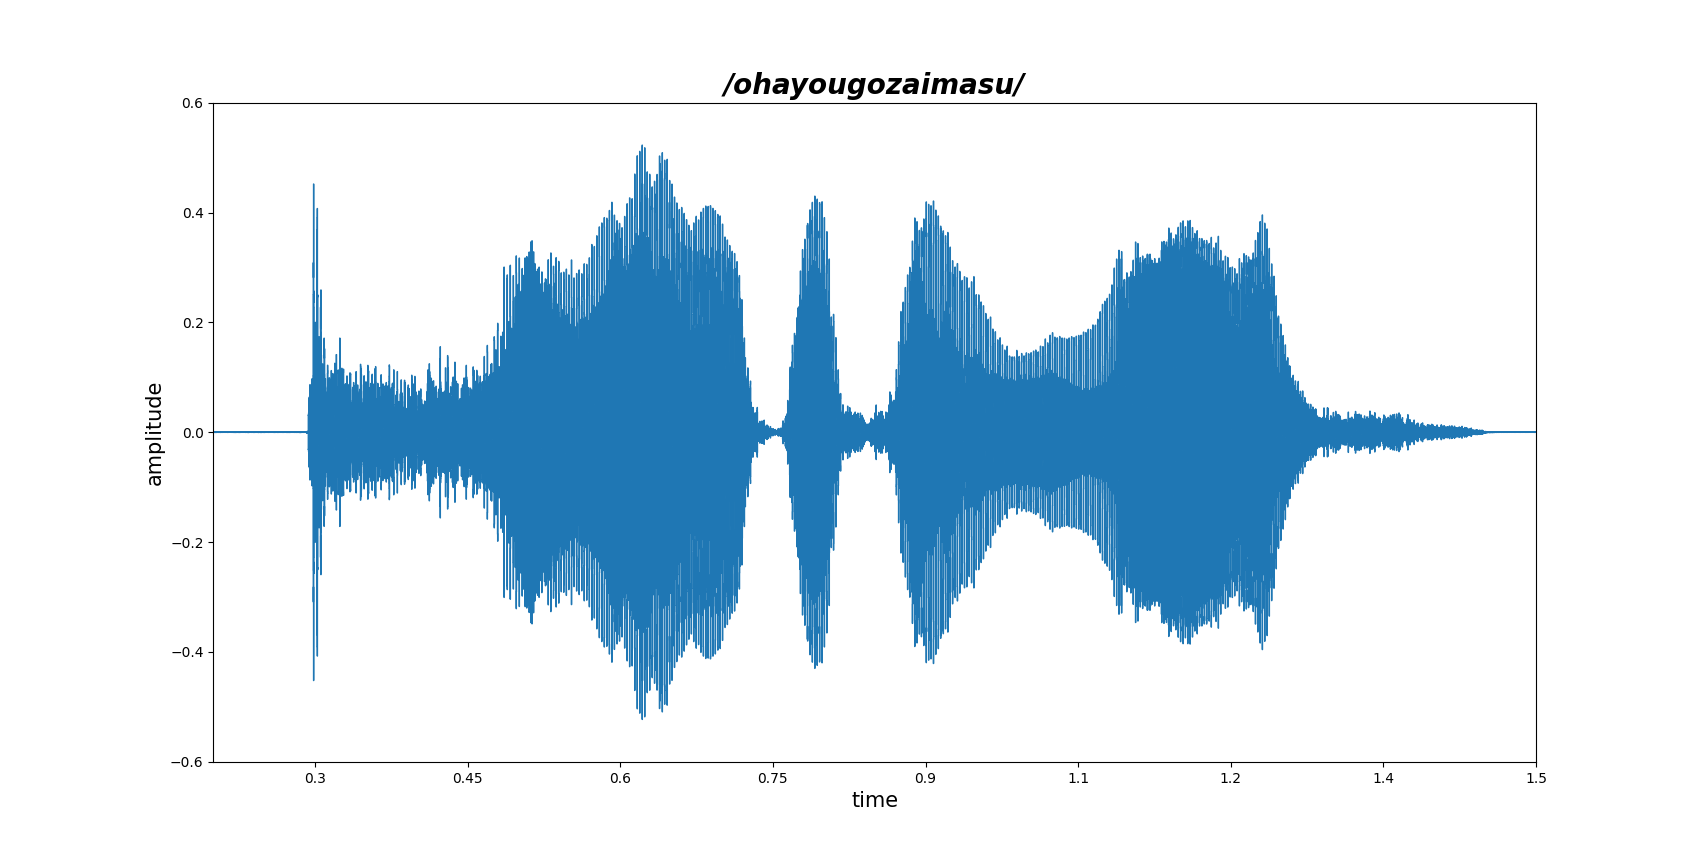
\includegraphics[width=100mm]{Figure_1.png}
        \caption{音声波形}
      \end{center}
    \end{figure}

    \newpage
    \textmc{
      次に、「おはようございます」という音声をSTFTで解析した結果が以下のものである。
      窓関数の信号点数は130点で、サンプル周波数は44100Hzである。よって、パワースペクトルの分解能は、
      約339Hzである。
    \\}

    \begin{lstlisting}
import scipy.io.wavfile as wio
import matplotlib.pyplot as plt

if __name__ == '__main__':
    rate, data = wio.read("./sample.wav")
    pxx, freqs, im, t = plt.specgram(data, Fs=rate, cmap="hsv", Fc=0, mode="psd", NFFT=130, scale="dB")
    plt.ylim(0, 20000)
    plt.show()
    plt.close()
    \end{lstlisting}

    \begin{figure}[h]
      \begin{center}
        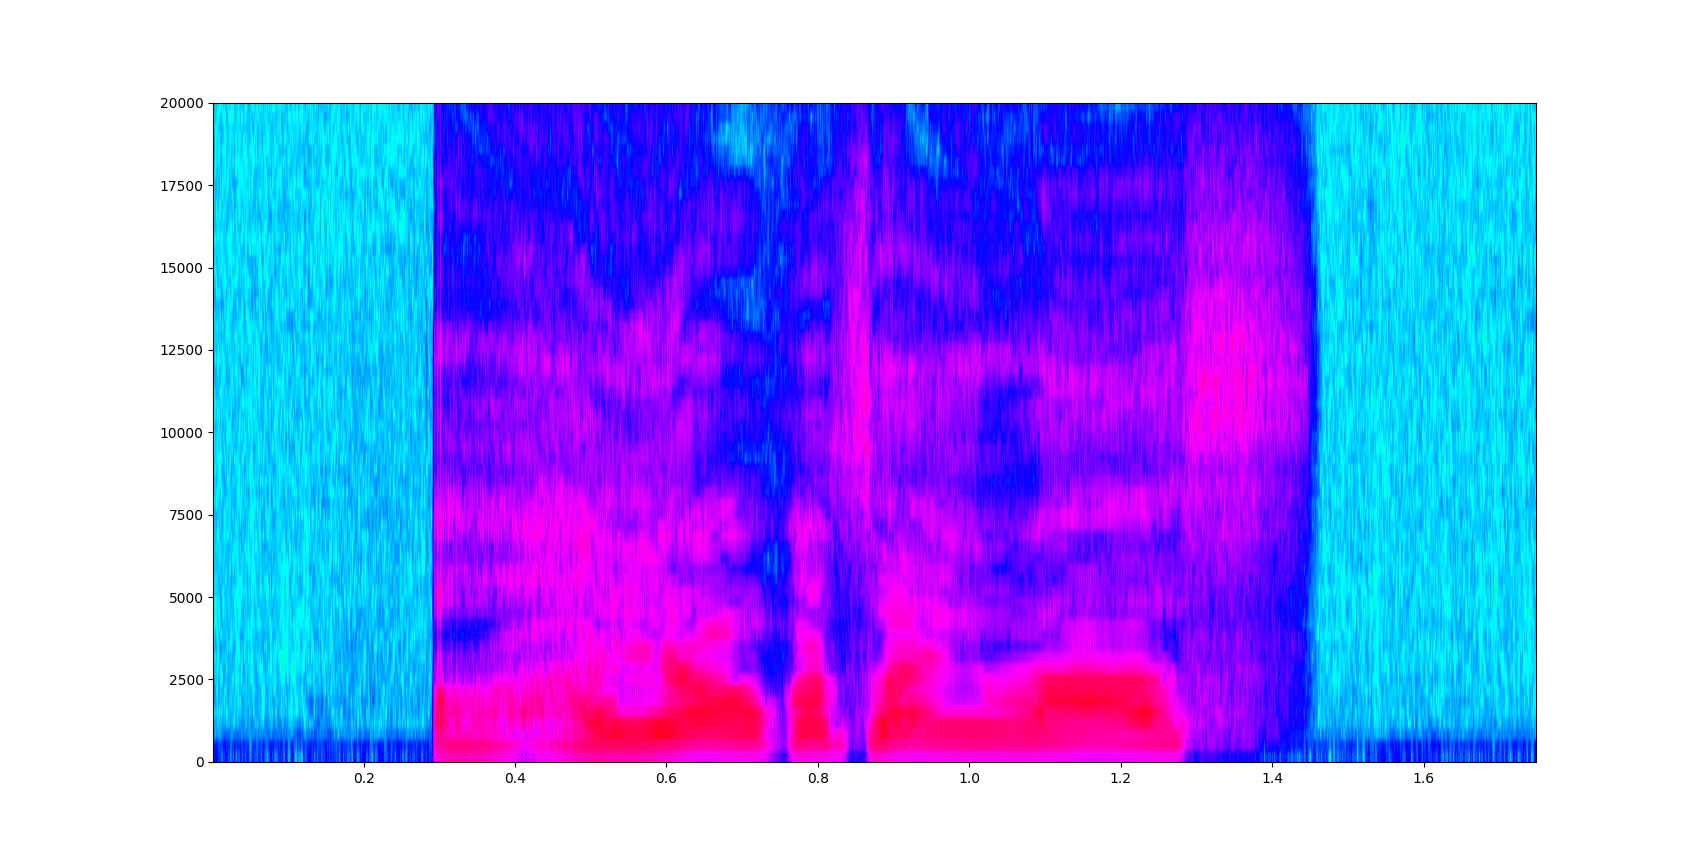
\includegraphics[width=100mm]{Figure_2.png}
        \caption{パワースペクトルの分解能: 約339Hz}
      \end{center}
    \end{figure}

    \newpage
    \textmc{
      窓関数の信号点数を10,000点に変更して解析を行ったパターンを以下に示す。
    \\}

    \begin{figure}[h]
      \begin{center}
        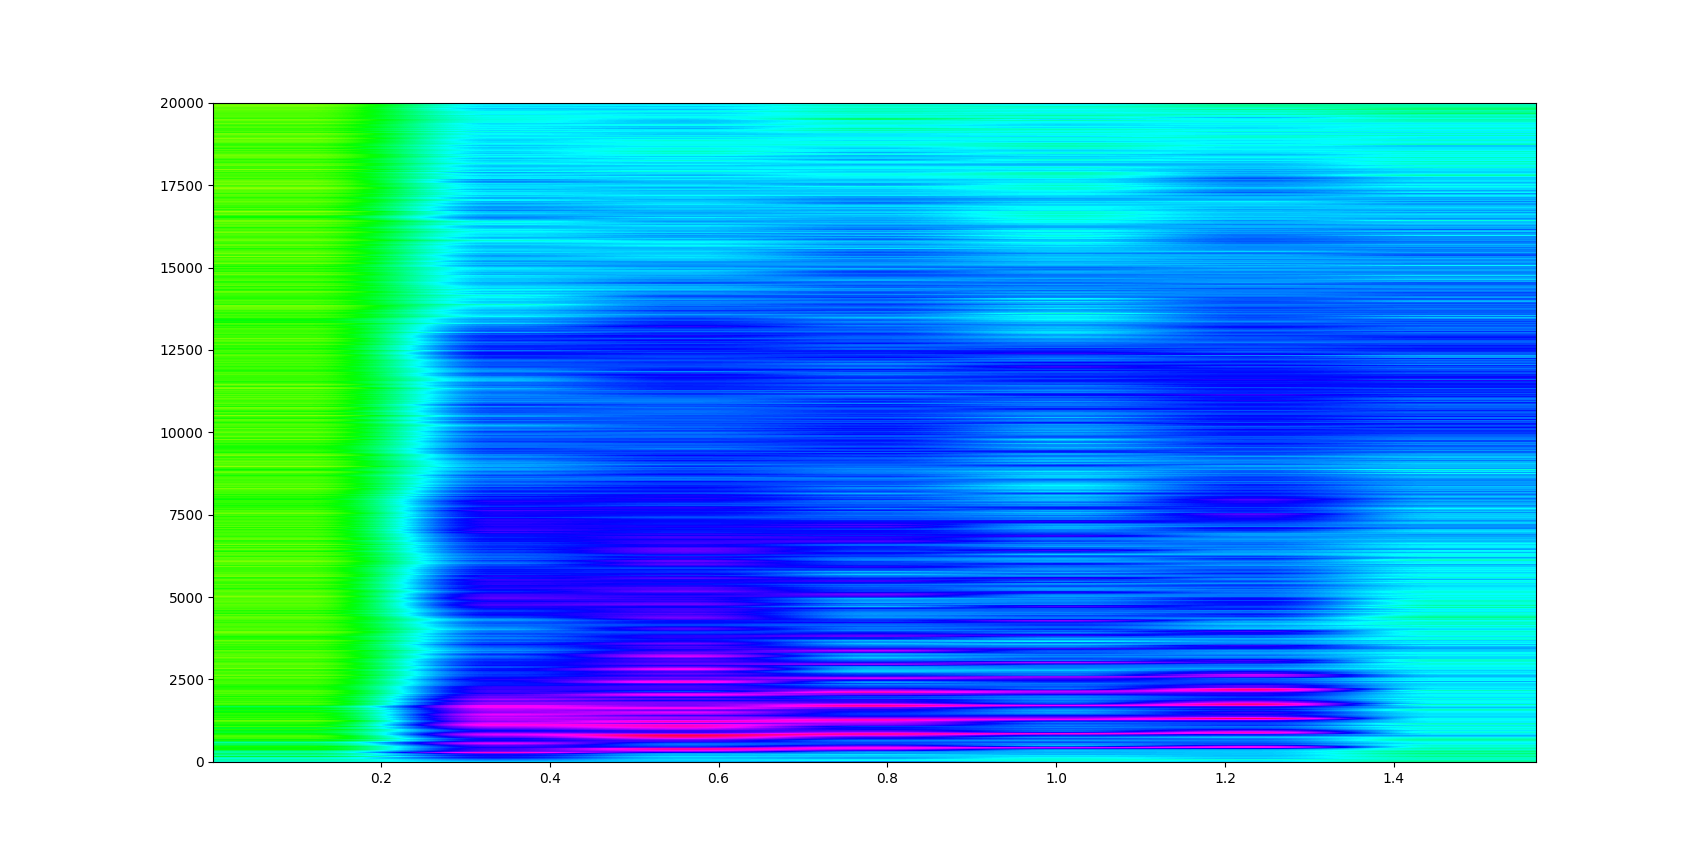
\includegraphics[width=100mm]{Figure_3.png}
        \caption{パワースペクトルの分解能: 約0.227Hz}
      \end{center}
    \end{figure}

    \textmc{
      上記の結果から分かるように、パワースペクトルの分解能が低いほどパワースペクトル密度の解析にノイズが強く入ることがわかる。
      \\}

  \textmc{\large \\}
  \textmc{\LARGE 第5回の講義についてのキーワード: 遺伝的アルゴリズム \\}
  \textmc{
    遺伝的アルゴリズムは、「1975年にミシガン大学の John Henry Holland によって提案された、生物の進化論を模した最適解を探索する最適化アルゴリズム」(参考文献[4]から引用)である。
    遺伝的アルゴリズムを適用できる分野は多くあり、自動作曲技術や画像生成などがある。
    遺伝的アルゴリズムは、自然淘汰→交叉+突然変異→次世代の発生のループで近似解の精度を上げていく。
    自然淘汰、交叉、突然変異それぞれに、様々な手法が考案されており、手法を変えることにより、より精度の良い結果を導くこともある。
    \\}
  \textmc{\large \\}
  \textmc{\LARGE 第6回の講義についてのキーワード: 自動運転レベル \\}
  \textmc{
    現在主流になっている自動運転レベルの基準は、アメリカの「自動運転技術会」(以下、SAEとする)の示したものである。
    レベルは六段階になっており、レベルゼロからレベル二までは、人間が主体、レベル三からレベル六までが、車が主体となっている。\\
    今回は、レベル一からレベル二の詳細について説明する。\\
    まず、レベル1については、このように定義されている。「運転自動化システムが動的運転タスクの縦方向又は横方向のいずれか(両方同時ではない)の車両運動制御のサブタスクを特定の限定領域において持続的に実行。この際、運転者は残りの動的運転タスクを実行する事が期待される」(参考文献[1]から引用)
    具体例としては、前走車に追従するACCなどがある。
    レベル2については、このように定義されている。「運転自動化システムが動的運転タスクの縦方向及び横方向両方の車両運動制御のサブタスクを特定の限定領域において持続的に実行。この際、運転者は動的運転タスクのサブタスクである対象物・事象の検知及び応答を完了し、システムを監督する事が期待される」(参考文献[1]から引用)
    具体例としては、「車間制御機能(車両の前後方向の自動制御)とレーンキーピングアシスト機能(車両の加減速制御)を同時に適用した運転支援」(参考文献[2]から引用)が上げられる。
    レベル3については、このように定義されている。「運転自動化システムが全ての動的運転タスクを限定領域において持続的に実行。この際、作動継続が困難な場合への応答準備ができている利用者は、他の車両のシステムにおける動的運転タスク実行システムに関連するシステム故障だけでなく、自動運転システムが出した介入の要求を受け容れ、適切に応答することが期待される」(参考文献[1]から引用)
    具体例としては、条件付きでハンズオフとアイズオフが許されていることが上げられる。
    \\}

    \begin{thebibliography}{99}
      \bibitem{自動運転LAB}自動運転レベルとは?(2023年最新版), \url{https://jidounten-lab.com/autonomous-level} \\
      \bibitem{Robot of Everything}自動運転レベル(Autonomous Driving level)の自動運転レベル2について, \url{https://www.zmp.co.jp/knowledge/ad_top/info/level2} \\
      \bibitem{大人の自動車保険}自動運転レベル3では何ができる?メリット・デメリットや搭載車種を紹介!, \url{https://www.ins-saison.co.jp/otona/oshiete/car/autonomous-driving-level3.html} \\
      \bibitem{CYBERNET}遺伝的アルゴリズムとは:遺伝的アルゴリズムの特徴から遺伝子の交叉と突然変異について解説, \url{https://www.cybernet.co.jp/optimus/tips/cae-optimization/detail/genetic_algorithm.html} \\
      \bibitem{もちおのブログ}pythonで時間周波数解析~STFT~, \url{https://heartstat.net/2018/11/13/python_stft/} \\
      \bibitem{Qiita}matplotlibのspecgram, \url{https://qiita.com/wataoka/items/3f01caaa85ae58ace4b0} \\
      \bibitem{Qiita}PythonによるSTFT等で利用する窓関数の比較, \url{https://qiita.com/uene/items/3501a439c5c4fb320153} \\
    \end{thebibliography}

\end{document}
